\documentclass[aspectratio=169,11pt]{beamer}

% Theme and colors - Standard academic style
\usetheme{Madrid}
\usecolortheme{default}

% Custom colors for slides
\definecolor{deepblue}{rgb}{0,0.2,0.6}
\definecolor{deepred}{rgb}{0.6,0,0}
\definecolor{deepgreen}{rgb}{0,0.5,0}

% VS Code Dark+ inspired color scheme for code
\definecolor{codebg}{HTML}{1E1E1E}
\definecolor{codefg}{HTML}{D4D4D4}
\definecolor{codekeyword}{HTML}{569CD6}
\definecolor{codestring}{HTML}{CE9178}
\definecolor{codecomment}{HTML}{6A9955}
\definecolor{codenumber}{HTML}{B5CEA8}
\definecolor{codefunction}{HTML}{DCDCAA}
\definecolor{codeparam}{HTML}{9CDCFE}
\definecolor{codeoperator}{HTML}{D4D4D4}
\definecolor{codetype}{HTML}{4EC9B0}
\definecolor{codedecorator}{HTML}{C586C0}
\definecolor{codeframe}{HTML}{3C3C3C}

% Packages
\usepackage{listings}
\usepackage{graphicx}
\usepackage{booktabs}
\usepackage{xcolor}
\usepackage{tikz}
\usepackage{pifont}  % For checkmarks and crosses
\usepackage{fancyvrb}

% Try to use fontspec if available (requires XeLaTeX/LuaLaTeX)
\usepackage{iftex}
\ifxetex
    \usepackage{fontspec}
    \setmonofont{JetBrains Mono}[Scale=0.85]
\else\ifluatex
    \usepackage{fontspec}
    \setmonofont{JetBrains Mono}[Scale=0.85]
\else
    % pdfLaTeX fallback
    \usepackage[T1]{fontenc}
    \usepackage{inconsolata}
\fi\fi

% Code listing styles - VS Code Dark+ theme
\lstdefinestyle{pythonstyle}{
    backgroundcolor=\color{codebg},
    basicstyle=\ttfamily\scriptsize\color{codefg},
    keywordstyle=\color{codekeyword}\bfseries,
    keywordstyle=[2]\color{codefunction},
    keywordstyle=[3]\color{codetype},
    stringstyle=\color{codestring},
    commentstyle=\color{codecomment}\itshape,
    numberstyle=\tiny\color{codenumber},
    breakatwhitespace=false,
    breaklines=true,
    captionpos=b,
    keepspaces=true,
    numbers=none,
    numbersep=5pt,
    showspaces=false,
    showstringspaces=false,
    showtabs=false,
    tabsize=4,
    frame=none,
    xleftmargin=5pt,
    xrightmargin=5pt,
    language=Python,
    morekeywords={self,True,False,None,as,with,yield,async,await},
    morekeywords=[2]{compile_model,QuantizationTransform,StaticQuantRule,CPrinter,DynamicQuantRuleMinMaxPerTensor,FuseDequantQuantPass,apply,generate_all,randn,relu,mean,forward,__init__},
    morekeywords=[3]{nn,torch,Module,Linear,Conv2d,BatchNorm2d,ReLU},
    texcl=false,
    mathescape=false,
    literate={->}{{\textcolor{codeoperator}{->}}}2
             {=}{{\textcolor{codeoperator}{=}}}1
}

\lstdefinestyle{cstyle}{
    backgroundcolor=\color{codebg},
    basicstyle=\ttfamily\scriptsize\color{codefg},
    keywordstyle=\color{codekeyword}\bfseries,
    keywordstyle=[2]\color{codefunction},
    stringstyle=\color{codestring},
    commentstyle=\color{codecomment}\itshape,
    numberstyle=\tiny\color{codenumber},
    breakatwhitespace=false,
    breaklines=true,
    captionpos=b,
    keepspaces=true,
    numbers=none,
    numbersep=5pt,
    showspaces=false,
    showstringspaces=false,
    showtabs=false,
    tabsize=4,
    frame=none,
    xleftmargin=5pt,
    xrightmargin=5pt,
    language=C,
    morekeywords=[2]{compute_dynamic_scale_int8,quantize_float_to_int8}
}

\lstdefinestyle{bashstyle}{
    backgroundcolor=\color{codebg},
    basicstyle=\ttfamily\scriptsize\color{codefg},
    keywordstyle=\color{codekeyword}\bfseries,
    commentstyle=\color{codecomment}\itshape,
    breaklines=true,
    frame=none,
    xleftmargin=5pt,
    xrightmargin=5pt,
    language=bash,
    morekeywords={python,pytest,src,examples,out}
}

\lstdefinestyle{diagramstyle}{
    backgroundcolor=\color{codebg},
    basicstyle=\ttfamily\scriptsize\color{codefg},
    breaklines=false,
    frame=none,
    xleftmargin=5pt,
    xrightmargin=5pt
}

\lstset{style=pythonstyle}

% Presentation info
\title[PyTorch-to-Quantized-C Compiler]{PyTorch-to-Quantized-C Compiler}
\subtitle{Compiling Neural Networks for Microcontrollers}
\author{Ashitabh Misra, Joydeep Bhattacharyya, Tarek Abdelzaher}
\institute{}
\date{\today}

% Navigation symbols
\setbeamertemplate{navigation symbols}{}

% Frame numbering
\setbeamertemplate{footline}{
    \leavevmode%
    \hbox{%
    \begin{beamercolorbox}[wd=0.5\paperwidth,ht=2.25ex,dp=1ex,left]{section in head/foot}%
        \usebeamerfont{section in head/foot}\hspace*{2ex}\insertsectionhead
    \end{beamercolorbox}%
    \begin{beamercolorbox}[wd=0.5\paperwidth,ht=2.25ex,dp=1ex,right]{page number in head/foot}%
        \usebeamerfont{page number in head/foot}\insertframenumber{} / \inserttotalframenumber\hspace*{2ex}
    \end{beamercolorbox}}%
    \vskip0pt%
}

\begin{document}

% Title slide
\begin{frame}
    \titlepage
\end{frame}

% Table of contents
\begin{frame}{Outline}
    \tableofcontents
\end{frame}

% Include sections
% ============================================================================
% SECTION 0: INTRODUCTION & MOTIVATION
% ============================================================================

\section{Introduction \& Motivation}

% ----------------------------------------------------------------------------
% Slide 0.1: The Problem
% ----------------------------------------------------------------------------
\begin{frame}{The Problem}
    \textbf{Deploying quantized neural networks on microcontrollers is challenging.}
    
    \vspace{1em}
    
    \textbf{Existing tools are inflexible and difficult to extend:}
    
    \begin{itemize}[<+->]
        \item \textbf{TFLite Micro:} Large binary size for microcontrollers usecases, not designed to be extended. As a result,
        extremely difficult to add new quantization techniques.
        
        \item \textbf{Glow:} Complex setup, designed for research not real-world embedded use, hard to add new features.
    \end{itemize}
\end{frame}

% ----------------------------------------------------------------------------
% Slide 0.2: Comparison with Existing Tools
% ----------------------------------------------------------------------------
\begin{frame}{Comparison with Existing Tools}
    \small
    \centering
    \begin{tabular}{l|ccc}
        \toprule
        \textbf{Feature} & \textbf{Tiny-NN-in-C} & \textbf{TFLite Micro} & \textbf{Glow} \\
        \midrule
        \uncover<2->{Framework} & \uncover<2->{PyTorch} & \uncover<2->{TensorFlow} & \uncover<2->{ONNX/PyTorch*} \\
        \uncover<3->{Output} & \uncover<3->{Standalone C} & \uncover<3->{.tflite + Interp.} & \uncover<3->{Compiled binary} \\
        \uncover<4->{Code Readability} & \uncover<5->{\color{deepgreen}\ding{51}} & \uncover<5->{\color{deepred}\ding{55} Binary} & \uncover<5->{\color{deepred}\ding{55} Opt. IR} \\
        \uncover<5->{Setup Complexity} & \uncover<6->{Simple (pip)} & \uncover<6->{Medium} & \uncover<6->{Complex} \\
        \uncover<6->{Binary Size} & \uncover<7->{$\sim$150KB} & \uncover<7->{$\sim$390KB+} & \uncover<7->{Varies} \\
        \uncover<7->{Quantization} & \uncover<8->{int8/16, mixed} & \uncover<8->{int8} & \uncover<8->{int8} \\
        \uncover<8->{Custom Rules} & \uncover<10->{\color{deepgreen}\ding{51} Regex} & \uncover<10->{\color{deepred}\ding{55} Per-layer} & \uncover<10->{\color{deepred}\ding{55} Manual} \\
        \uncover<9->{Extensibility} & \uncover<12->{\color{deepgreen}\ding{51} Easy} & \uncover<12->{\color{deepred}\ding{55} C++} & \uncover<12->{\color{deepred}\ding{55} LLVM} \\
        \uncover<10->{Transparency} & \uncover<14->{\color{deepgreen}\ding{51} See code} & \uncover<14->{\color{deepred}\ding{55} Black box} & \uncover<14->{\color{deepred}\ding{55} Black box} \\
        \bottomrule
    \end{tabular}
    
    \vspace{0.5em}
    \uncover<12->{\footnotesize *Glow development has slowed; PyTorch support via ONNX conversion}
\end{frame}

% ----------------------------------------------------------------------------
% Slide 0.3: Architecture Comparison - TFLite Micro
% ----------------------------------------------------------------------------
\begin{frame}{Architecture Comparison}
    \textbf{TFLite Micro:}
    \begin{center}
    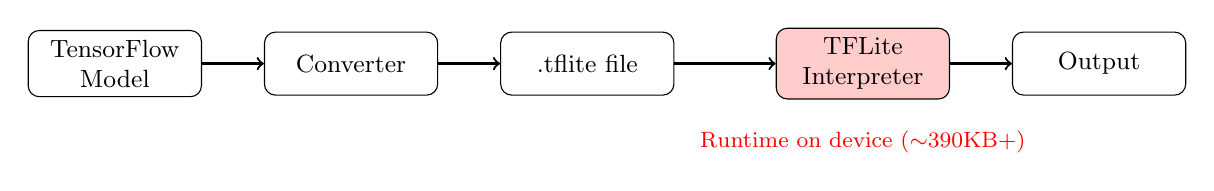
\begin{tikzpicture}[
        box/.style={draw, rounded corners, minimum width=2.2cm, minimum height=0.8cm, align=center, font=\small},
        arrow/.style={->, thick}
    ]
        \onslide<1->{
            \node[box] (tf) at (0,0) {TensorFlow\\Model};
        }
        \onslide<2->{
            \node[box] (conv) at (3,0) {Converter};
            \draw[arrow] (tf) -- (conv);
        }
        \onslide<3->{
            \node[box] (tflite) at (6,0) {.tflite file};
            \draw[arrow] (conv) -- (tflite);
        }
        \onslide<4->{
            \node[box, fill=red!20] (interp) at (9.5,0) {TFLite\\Interpreter};
            \draw[arrow] (tflite) -- (interp);
        }
        \onslide<5->{
            \node[box] (out) at (12.5,0) {Output};
            \draw[arrow] (interp) -- (out);
        }
        \onslide<6->{
            \node[font=\footnotesize, text=red] at (9.5,-1) {Runtime on device ($\sim$390KB+)};
        }
    \end{tikzpicture}
    \end{center}
    
    \vspace{1em}
    
    \onslide<7->{
    \textbf{Glow:}
    \begin{center}
    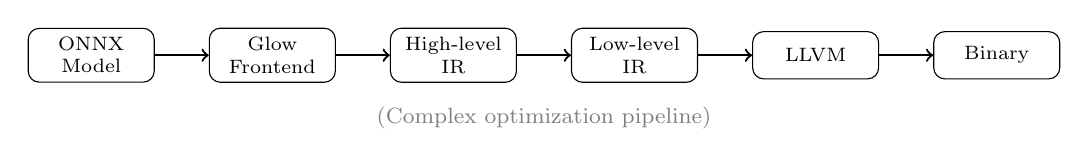
\begin{tikzpicture}[
        box/.style={draw, rounded corners, minimum width=1.6cm, minimum height=0.6cm, align=center, font=\scriptsize},
        arrow/.style={->, thick}
    ]
        \node[box] (onnx) at (0,0) {ONNX\\Model};
        \node[box] (front) at (2.3,0) {Glow\\Frontend};
        \node[box] (hir) at (4.6,0) {High-level\\IR};
        \node[box] (lir) at (6.9,0) {Low-level\\IR};
        \node[box] (llvm) at (9.2,0) {LLVM};
        \node[box] (bin) at (11.5,0) {Binary};
        
        \draw[arrow] (onnx) -- (front);
        \draw[arrow] (front) -- (hir);
        \draw[arrow] (hir) -- (lir);
        \draw[arrow] (lir) -- (llvm);
        \draw[arrow] (llvm) -- (bin);
        
        \node[font=\footnotesize, text=gray] at (5.75,-0.8) {(Complex optimization pipeline)};
    \end{tikzpicture}
    \end{center}
    }
\end{frame}

% ----------------------------------------------------------------------------
% Slide 0.4: Architecture Comparison - Tiny-NN-in-C
% ----------------------------------------------------------------------------
\begin{frame}{Our Approach: Tiny-NN-in-C}
    \begin{center}
    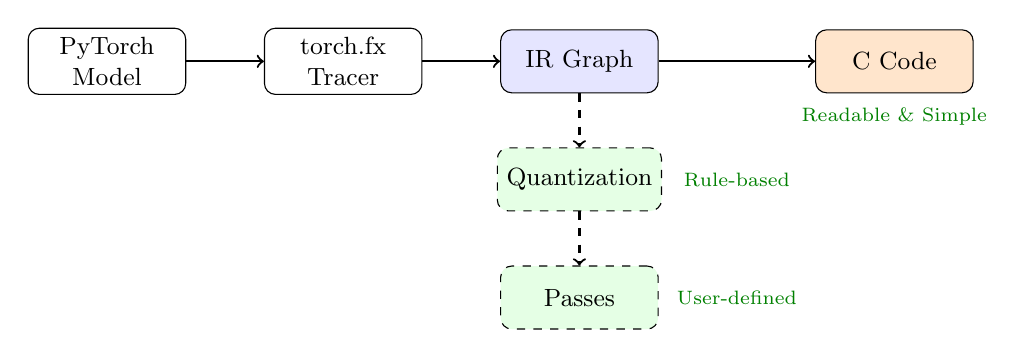
\begin{tikzpicture}[
        box/.style={draw, rounded corners, minimum width=2cm, minimum height=0.8cm, align=center, font=\small},
        optbox/.style={draw, rounded corners, dashed, minimum width=2cm, minimum height=0.8cm, align=center, font=\small, fill=green!10},
        arrow/.style={->, thick},
        optarrow/.style={->, thick, dashed}
    ]
        \onslide<1->{
            \node[box] (pytorch) at (0,0) {PyTorch\\Model};
        }
        \onslide<2->{
            \node[box] (fx) at (3,0) {torch.fx\\Tracer};
            \draw[arrow] (pytorch) -- (fx);
        }
        \onslide<3->{
            \node[box, fill=blue!10] (ir) at (6,0) {IR Graph};
            \draw[arrow] (fx) -- (ir);
        }
        \onslide<4->{
            \node[optbox] (quant) at (6,-1.5) {Quantization};
            \draw[optarrow] (ir) -- (quant);
            \node[font=\scriptsize, text=deepgreen] at (8,-1.5) {Rule-based};
        }
        \onslide<5->{
            \node[optbox] (passes) at (6,-3) {Passes};
            \draw[optarrow] (quant) -- (passes);
            \node[font=\scriptsize, text=deepgreen] at (8,-3) {User-defined};
        }
        \onslide<6->{
            \node[box, fill=orange!20] (ccode) at (10,0) {C Code};
            \draw[arrow] (ir) -- (ccode);
            \node[font=\scriptsize, text=deepgreen] at (10,-0.7) {Readable \& Simple};
        }
    \end{tikzpicture}
    \end{center}
    
    \vspace{1em}
    
    \onslide<7->{
        \begin{block}{Key Insight}
            We achieve \textbf{transparency} and \textbf{simplicity} with minimal performance penalty.
        \end{block}
    }
\end{frame}


% ============================================================================
% SECTION 1: TUTORIAL & USE CASES
% ============================================================================

\section{Tutorial \& Use Cases}

% ----------------------------------------------------------------------------
% Slide 1.0: Quick Start - The Core API
% ----------------------------------------------------------------------------
\begin{frame}[fragile]{Quick Start: The Core API}
    \textbf{Three simple steps to compile a quantized model:}
    \vspace{0.5em}

\onslide<1->
    \textbf{Step 1: Compile to C (float)}
\begin{lstlisting}[style=pythonstyle]
from src.pytorch_to_c.compiler import compile_model

ir_graph = compile_model(model, example_input, output_dir="out/")
\end{lstlisting}

\onslide<2->
    \vspace{0.5em}
    \textbf{Step 2: Define quantization rules}
\begin{lstlisting}[style=pythonstyle]
from src.pytorch_to_c.quantization import StaticQuantRule

rules = [StaticQuantRule(pattern=r'fc.*', dtype='int8', ...)]
\end{lstlisting}

\onslide<3->
    \vspace{0.5em}
    \textbf{Step 3: Apply quantization and generate}
\begin{lstlisting}[style=pythonstyle]
transform = QuantizationTransform(rules)
quant_ir = transform.apply(ir_graph)
CPrinter(quant_ir).generate_all("out/")
\end{lstlisting}

\end{frame}

% \begin{onlyenv}<4>
%     \textbf{Complete workflow:}
% \begin{lstlisting}[style=pythonstyle]
% ir_graph = compile_model(model, example_input, return_ir=True)
% rules = [StaticQuantRule(pattern=r'fc.*', dtype='int8', ...)]
% quant_ir = QuantizationTransform(rules).apply(ir_graph)
% CPrinter(quant_ir).generate_all("out/")
% \end{lstlisting}
% \end{onlyenv}
% \end{frame}

% ----------------------------------------------------------------------------
% Slide 1.1: What is This?
% ----------------------------------------------------------------------------
\begin{frame}[fragile]{What is This?}
    \textbf{A PyTorch-to-C compiler for microcontrollers}
    
    \vspace{0.5em}
    
    \begin{itemize}[<+->]
        \item Takes PyTorch models $\rightarrow$ Generates standalone C code
        \item Supports quantization (int8, int16) for embedded deployment
        \item Extensible rule-based system for selective quantization
        \item IR-based architecture enables optimization passes
    \end{itemize}
    
    \vspace{1em}
    
\begin{uncoverenv}<5->
\begin{lstlisting}[style=bashstyle]
python examples/tiny_resnet.py
\end{lstlisting}
\end{uncoverenv}
\end{frame}

% ----------------------------------------------------------------------------
% Slide 1.2a: Simple MLP Example - Init
% ----------------------------------------------------------------------------
\begin{frame}[fragile]{Simple MLP Example}
    \textbf{Model:} 2-layer MLP (Linear $\rightarrow$ ReLU $\rightarrow$ Linear)
    
\begin{lstlisting}[style=pythonstyle]
class SimpleMLP(nn.Module):
    def __init__(self, input_size=784, hidden_size=128, output_size=10):
        super().__init__()
\end{lstlisting}
\end{frame}

% ----------------------------------------------------------------------------
% Slide 1.2b: Simple MLP Example - Layers
% ----------------------------------------------------------------------------
\begin{frame}[fragile]{Simple MLP Example}
    \textbf{Model:} 2-layer MLP (Linear $\rightarrow$ ReLU $\rightarrow$ Linear)
    
\begin{lstlisting}[style=pythonstyle]
class SimpleMLP(nn.Module):
    def __init__(self, input_size=784, hidden_size=128, output_size=10):
        super().__init__()
        self.fc1 = nn.Linear(input_size, hidden_size)
        self.relu = nn.ReLU()
        self.fc2 = nn.Linear(hidden_size, output_size)
\end{lstlisting}
\end{frame}

% ----------------------------------------------------------------------------
% Slide 1.2c: Simple MLP Example - Forward
% ----------------------------------------------------------------------------
\begin{frame}[fragile]{Simple MLP Example}
    \textbf{Model:} 2-layer MLP (Linear $\rightarrow$ ReLU $\rightarrow$ Linear)
    
\begin{lstlisting}[style=pythonstyle]
class SimpleMLP(nn.Module):
    def __init__(self, input_size=784, hidden_size=128, output_size=10):
        super().__init__()
        self.fc1 = nn.Linear(input_size, hidden_size)
        self.relu = nn.ReLU()
        self.fc2 = nn.Linear(hidden_size, output_size)
    
    def forward(self, x):
        x = self.fc1(x)
        x = self.relu(x)
        x = self.fc2(x)
        return x
\end{lstlisting}
\end{frame}

% ----------------------------------------------------------------------------
% Slide 1.2d: Simple MLP Example - Compile
% ----------------------------------------------------------------------------
\begin{frame}[fragile]{Simple MLP Example}
    \textbf{Compile to C:}
    
\begin{lstlisting}[style=pythonstyle]
model = SimpleMLP(input_size=784, hidden_size=128, output_size=10)
example_input = torch.randn(1, 784)

ir_graph = compile_model(
    model=model,
    example_input=example_input,
    output_dir="generated"
)
\end{lstlisting}
\end{frame}

% ----------------------------------------------------------------------------
% Slide 1.2e: Simple MLP Example - Generated IR
% ----------------------------------------------------------------------------
\begin{frame}[fragile]{Simple MLP Example: Generated IR Graph}
    \textbf{IR Graph structure:}
    
\begin{lstlisting}[style=diagramstyle]
IRGraph:
  Inputs: ['x']
  Outputs: ['fc2']
  Parameters: ['fc1_weight', 'fc1_bias', 'fc2_weight', 'fc2_bias']
  Nodes:
    x [input]
      inputs: []
      users: [fc1]
      shape: (1, 784), dtype: float32
    fc1 [linear]
      inputs: [x]
      users: [relu]
      shape: (1, 128), dtype: float32
    relu [relu]
      inputs: [fc1]
      users: [fc2]
      shape: (1, 128), dtype: float32
    fc2 [linear]
      inputs: [relu]
      users: []
      shape: (1, 10), dtype: float32
\end{lstlisting}
\end{frame}

% ----------------------------------------------------------------------------
% Slide 1.3a: ResNet-Style Model - Block Init
% ----------------------------------------------------------------------------
\begin{frame}[fragile]{ResNet-Style Model (Skip Connections)}
    \textbf{Architecture:} Conv $\rightarrow$ BatchNorm $\rightarrow$ ReLU $\rightarrow$ Skip $\rightarrow$ Pool $\rightarrow$ FC
    
\begin{lstlisting}[style=pythonstyle]
class ResNetBlock(nn.Module):
    def __init__(self, channels):
        super().__init__()
        self.conv1 = nn.Conv2d(channels, channels, 3, padding=1)
        self.bn1 = nn.BatchNorm2d(channels)
\end{lstlisting}
\end{frame}

% ----------------------------------------------------------------------------
% Slide 1.3b: ResNet-Style Model - Block Forward
% ----------------------------------------------------------------------------
\begin{frame}[fragile]{ResNet-Style Model (Skip Connections)}
    \textbf{Architecture:} Conv $\rightarrow$ BatchNorm $\rightarrow$ ReLU $\rightarrow$ Skip $\rightarrow$ Pool $\rightarrow$ FC
    
\begin{lstlisting}[style=pythonstyle]
class ResNetBlock(nn.Module):
    def __init__(self, channels):
        super().__init__()
        self.conv1 = nn.Conv2d(channels, channels, 3, padding=1)
        self.bn1 = nn.BatchNorm2d(channels)
    
    def forward(self, x):
        identity = x
        out = torch.relu(self.bn1(self.conv1(x)))
        return out + identity
\end{lstlisting}
\end{frame}

% ----------------------------------------------------------------------------
% Slide 1.3c: ResNet-Style Model - Full Model
% ----------------------------------------------------------------------------
\begin{frame}[fragile]{ResNet-Style Model (Skip Connections)}
    \textbf{TinyResNet:} Using ResNetBlock with skip connections
    
\begin{lstlisting}[style=pythonstyle]
class TinyResNet(nn.Module):
    def __init__(self):
        super().__init__()
        self.conv_init = nn.Conv2d(3, 32, 3, padding=1)
        self.block1 = ResNetBlock(32)
        self.fc = nn.Linear(32, 10)
    
    def forward(self, x):
        x = torch.relu(self.conv_init(x))
        x = self.block1(x)
        x = x.mean(dim=[2, 3])
        return self.fc(x)
\end{lstlisting}
\end{frame}

% ----------------------------------------------------------------------------
% Slide 1.4a: Static Quantization - Define Rule
% ----------------------------------------------------------------------------
\begin{frame}[fragile]{Static Quantization}
    \textbf{Key idea:} Scales are known at compile time (from calibration)
    
    \vspace{0.5em}
    \textbf{Step 1: Define quantization rules}
    
\begin{lstlisting}[style=pythonstyle]
from src.pytorch_to_c.quantization import StaticQuantRule

rules = [
    StaticQuantRule(
        pattern=r'fc.*',
        dtype='int8',
\end{lstlisting}
\end{frame}

% ----------------------------------------------------------------------------
% Slide 1.4b: Static Quantization - Complete Rule
% ----------------------------------------------------------------------------
\begin{frame}[fragile]{Static Quantization}
    \textbf{Key idea:} Scales are known at compile time (from calibration)
    
    \vspace{0.5em}
    \textbf{Step 1: Define quantization rules}
    
\begin{lstlisting}[style=pythonstyle]
from src.pytorch_to_c.quantization import StaticQuantRule

rules = [
    StaticQuantRule(
        pattern=r'fc.*',
        dtype='int8',
        input_scale=0.01, weight_scale=0.01, output_scale=0.01
    )
]
\end{lstlisting}
\end{frame}

% ----------------------------------------------------------------------------
% Slide 1.4c: Static Quantization - Apply
% ----------------------------------------------------------------------------
\begin{frame}[fragile]{Static Quantization}
    \textbf{Key idea:} Scales are known at compile time (from calibration)
    
    \vspace{0.5em}
    \textbf{Step 2: Apply to IR graph}
    
\begin{lstlisting}[style=pythonstyle]
ir_graph = compile_model(model, example_input, return_ir=True)
transform = QuantizationTransform(rules)
quant_ir = transform.apply(ir_graph)
\end{lstlisting}
\end{frame}

% ----------------------------------------------------------------------------
% Slide 1.5a: Dynamic Quantization - Rule
% ----------------------------------------------------------------------------
\begin{frame}[fragile]{Dynamic Quantization}
    \textbf{Key idea:} Input scale computed at runtime from actual data
    
    \vspace{0.5em}
    \textbf{Define dynamic rule (no calibration needed!):}
    
\begin{lstlisting}[style=pythonstyle]
from src.pytorch_to_c.quantization import DynamicQuantRuleMinMaxPerTensor

rules = [
    DynamicQuantRuleMinMaxPerTensor(
        pattern=r'fc.*',
        dtype='int8'
    )
]
\end{lstlisting}
\end{frame}

% ----------------------------------------------------------------------------
% Slide 1.5b: Dynamic Quantization - Generated C
% ----------------------------------------------------------------------------
\begin{frame}[fragile]{Dynamic Quantization}
    \textbf{Key idea:} Input scale computed at runtime from actual data
    
    \vspace{0.5em}
    \textbf{Generated C code computes scale dynamically:}
    
\begin{lstlisting}[style=cstyle]
float scale = compute_dynamic_scale_int8(input, 784);
quantize_float_to_int8(input, 784, scale, 0, buf_quantized);
\end{lstlisting}

    \vspace{1em}
    
    \begin{block}{Advantage}
        No calibration dataset required---scales derived from weight statistics.
    \end{block}
\end{frame}

% ----------------------------------------------------------------------------
% Slide 1.6a: Mixed Precision - Encoder
% ----------------------------------------------------------------------------
\begin{frame}[fragile]{Mixed Precision Quantization}
    \textbf{Selective quantization:} Different rules for different layers
    
\begin{lstlisting}[style=pythonstyle]
rules = [
    StaticQuantRule(pattern=r'.*encoder.*', dtype='int8', ...),
]
\end{lstlisting}
\end{frame}

% ----------------------------------------------------------------------------
% Slide 1.6b: Mixed Precision - Encoder + Output
% ----------------------------------------------------------------------------
\begin{frame}[fragile]{Mixed Precision Quantization}
    \textbf{Selective quantization:} Different rules for different layers
    
\begin{lstlisting}[style=pythonstyle]
rules = [
    StaticQuantRule(pattern=r'.*encoder.*', dtype='int8', ...),
    
    StaticQuantRule(pattern=r'.*output.*', dtype='int16', ...),
]
\end{lstlisting}
    
\end{frame}


% ----------------------------------------------------------------------------
% Slide 1.7: Quantization Results
% ----------------------------------------------------------------------------
\begin{frame}{Correctness Results (On TinyResNet model)}
    
    \textbf{Comparing our implementation with Pytorch Float32 model.}
    \centering
    \begin{tabular}{lcc}
        \toprule
        \textbf{Configuration} & \textbf{Max Error} & \textbf{Memory Savings} \\
        \midrule
        \uncover<2->{Float32 (baseline)} & \uncover<2->{$1.19 \times 10^{-7}$} & \uncover<2->{---} \\
        \uncover<3->{Static int16} & \uncover<3->{0.07\%} & \uncover<3->{2$\times$} \\
        \uncover<4->{Static int8} & \uncover<4->{1.63\%} & \uncover<4->{4$\times$} \\
        \uncover<5->{Dynamic int8} & \uncover<5->{2.95\%} & \uncover<5->{4$\times$} \\
        \bottomrule
    \end{tabular}
    
    \vspace{1em}
    
    \uncover<6->{
        \begin{block}{Takeaway}
            Choose precision based on your accuracy requirements and memory constraints.
        \end{block}
    }
\end{frame}

% ----------------------------------------------------------------------------
% Slide 1.8a: FuseDequantQuant - Before
% ----------------------------------------------------------------------------
\begin{frame}[fragile]{Optimization Pass: FuseDequantQuant}
    \textbf{Problem:} Consecutive quantized layers have redundant conversions
    
\begin{lstlisting}[style=diagramstyle]
BEFORE: fc1(int8) -> dequant(float) -> quant(int8) -> fc2(int8)
\end{lstlisting}
\end{frame}

% ----------------------------------------------------------------------------
% Slide 1.8b: FuseDequantQuant - After
% ----------------------------------------------------------------------------
\begin{frame}[fragile]{Optimization Pass: FuseDequantQuant}
    \textbf{Problem:} Consecutive quantized layers have redundant conversions
    
\begin{lstlisting}[style=diagramstyle]
BEFORE: fc1(int8) -> dequant(float) -> quant(int8) -> fc2(int8)
AFTER:  fc1(int8) -> fc2(int8)
\end{lstlisting}
\end{frame}

% ----------------------------------------------------------------------------
% Slide 1.8c: FuseDequantQuant - Code
% ----------------------------------------------------------------------------
\begin{frame}[fragile]{Optimization Pass: FuseDequantQuant}
    \textbf{Apply the optimization pass:}
    
\begin{lstlisting}[style=pythonstyle]
from src.passes import FuseDequantQuantPass

fuse_pass = FuseDequantQuantPass()
optimized_ir = fuse_pass.apply(quant_ir)
\end{lstlisting}
\end{frame}

% ----------------------------------------------------------------------------
% Slide 1.8d: FuseDequantQuant - Result
% ----------------------------------------------------------------------------
\begin{frame}[fragile]{Optimization Pass: FuseDequantQuant}
    \textbf{Apply the optimization pass:}
    
\begin{lstlisting}[style=pythonstyle]
from src.passes import FuseDequantQuantPass

fuse_pass = FuseDequantQuantPass()
optimized_ir = fuse_pass.apply(quant_ir)
\end{lstlisting}

    \vspace{0.5em}
    
    \begin{alertblock}{Result}
        When scales match, fusion is \textbf{bit-identical}: Max error = \texttt{0.00e+00}
    \end{alertblock}
\end{frame}

% ============================================================================
% SECTION 2: INNER WORKINGS
% ============================================================================

\section{Inner Workings}

% ----------------------------------------------------------------------------
% Slide 2.1: Architecture Overview
% ----------------------------------------------------------------------------
\begin{frame}{Architecture Overview}
    \begin{center}
    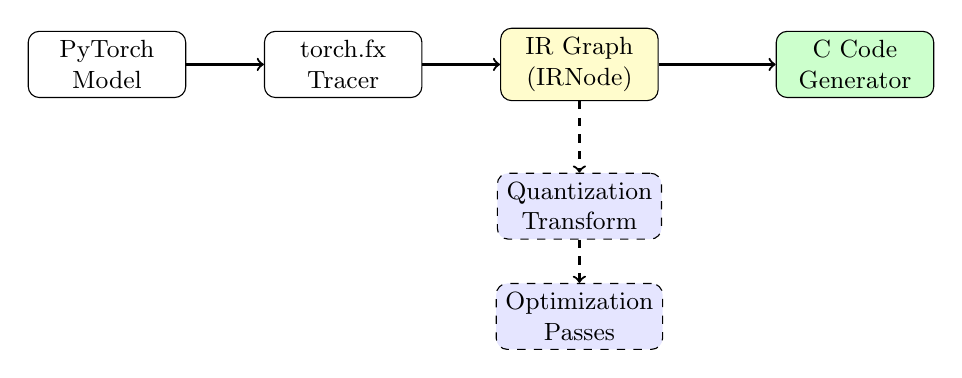
\begin{tikzpicture}[
        box/.style={draw, rounded corners, minimum width=2cm, minimum height=0.8cm, align=center, font=\small},
        optbox/.style={draw, rounded corners, dashed, minimum width=2cm, minimum height=0.8cm, align=center, font=\small, fill=blue!10},
        arrow/.style={->, thick}
    ]
        \node[box] (pytorch) at (0,0) {PyTorch\\Model};
        \node[box] (fx) at (3,0) {torch.fx\\Tracer};
        \node[box, fill=yellow!20] (ir) at (6,0) {IR Graph\\(IRNode)};
        \node[box, fill=green!20] (ccode) at (9.5,0) {C Code\\Generator};
        
        \draw[arrow] (pytorch) -- (fx);
        \draw[arrow] (fx) -- (ir);
        \draw[arrow] (ir) -- (ccode);
        
        \node[optbox] (quant) at (6,-1.8) {Quantization\\Transform};
        \node[optbox] (passes) at (6,-3.2) {Optimization\\Passes};
        
        \draw[arrow, dashed] (ir) -- (quant);
        \draw[arrow, dashed] (quant) -- (passes);
    \end{tikzpicture}
    \end{center}
    
    \vspace{0.5em}
    
    \textbf{Key files:}
    \begin{itemize}
        \item \texttt{frontend/fx\_tracer.py} -- torch.fx tracing
        \item \texttt{lowering/lower.py} -- FX $\rightarrow$ IR conversion
        \item \texttt{ir/graph.py} -- IR graph structure
        \item \texttt{codegen/c\_printer.py} -- C code generation
    \end{itemize}
\end{frame}

% ----------------------------------------------------------------------------
% Slide 2.2: IR Node Structure
% ----------------------------------------------------------------------------
\begin{frame}[fragile]{IR Node Structure}
    \textbf{Base class:} \texttt{src/pytorch\_to\_c/ir/node.py}
    
\begin{lstlisting}[style=pythonstyle]
class IRNode:
    def __init__(self, name, op_type, inputs=None, dtype='float32'):
        self.name = name           # Unique identifier
        self.op_type = op_type     # 'linear', 'conv2d', 'relu', etc.
        self.inputs = inputs or [] # List of input IRNodes
        self.users = []            # Nodes that use this output
        self.dtype = dtype         # 'float32', 'int8', 'int16'
        self.output_shape = None   # Inferred shape
        self.metadata = {}         # Extra info (weights, etc.)
    
    def get_c_dtype(self) -> str:
        """Returns C type: 'float', 'int8_t', 'int16_t'"""
\end{lstlisting}

    \vspace{0.5em}
    \textbf{Graph is doubly-linked:} \texttt{inputs} + \texttt{users} enable traversal in both directions
\end{frame}

% ----------------------------------------------------------------------------
% Slide 2.3: IR Graph Structure
% ----------------------------------------------------------------------------
\begin{frame}[fragile]{IR Graph Structure}
    \textbf{File:} \texttt{src/pytorch\_to\_c/ir/graph.py}
    
    \begin{columns}
    \begin{column}{0.5\textwidth}
\begin{lstlisting}[style=pythonstyle]
class IRGraph:
    def __init__(self):
        self.nodes = []
        self.inputs = []
        self.outputs = []
        self.parameters = {}
    
    def print_graph(self):
        """Pretty-print graph"""
\end{lstlisting}
    \end{column}
    \begin{column}{0.5\textwidth}
        \textbf{Example IR output:}
\begin{lstlisting}[style=diagramstyle]
x [input] dtype=float32
  inputs: []
  users: [fc1]
fc1 [linear] dtype=float32
  inputs: [x]
  users: [relu]
  shape: (1, 8)
\end{lstlisting}
    \end{column}
    \end{columns}
\end{frame}

% ----------------------------------------------------------------------------
% Slide 2.4: Quantization Rule System
% ----------------------------------------------------------------------------
\begin{frame}[fragile]{Quantization Rule System}
    \textbf{Base class:} \texttt{src/pytorch\_to\_c/quantization/rules.py}
    
\begin{lstlisting}[style=pythonstyle]
class QuantRule(ABC):
    def __init__(self, pattern: str, dtype: str):
        self.pattern = re.compile(pattern)  # Regex for layer names
        self.dtype = dtype                   # 'int8' or 'int16'
    
    def matches(self, node: IRNode) -> bool:
        """Check if rule applies to this node"""
        return self.pattern.search(node.name) is not None
    
    @abstractmethod
    def create_quant_node(self, float_node: IRNode) -> QuantIRNode:
        """Create quantized version of the node"""
\end{lstlisting}

    \vspace{0.5em}
    \textbf{Rule matching:} First matching rule wins
\begin{lstlisting}[style=pythonstyle]
RuleMatcher([rule1, rule2, rule3])  # Checked in order
\end{lstlisting}
\end{frame}

% ----------------------------------------------------------------------------
% Slide 2.5: Writing a Custom Rule
% ----------------------------------------------------------------------------
\begin{frame}[fragile]{Writing a Custom Rule}
    \textbf{Example: Static Quantization Rule}
    
\begin{onlyenv}<1>
\begin{lstlisting}[style=pythonstyle]
class StaticQuantRule(QuantRule):
    def __init__(self, pattern, dtype, 
                 input_scale, weight_scale, output_scale, ...):
        super().__init__(pattern, dtype)
        self.input_scale = input_scale
        # ... store all scales/offsets
\end{lstlisting}
\end{onlyenv}

\begin{onlyenv}<2>
\begin{lstlisting}[style=pythonstyle]
class StaticQuantRule(QuantRule):
    def __init__(self, pattern, dtype, 
                 input_scale, weight_scale, output_scale, ...):
        super().__init__(pattern, dtype)
        self.input_scale = input_scale
    
    def create_quant_node(self, float_node: IRNode) -> QuantIRNode:
        if float_node.op_type == 'linear':
            return StaticQuantLinearNode(
                name=float_node.name, dtype=self.dtype,
                input_scale=self.input_scale, ...
            )
        elif float_node.op_type == 'conv2d':
            return StaticQuantConv2dNode(...)
\end{lstlisting}
\end{onlyenv}
\end{frame}

% ----------------------------------------------------------------------------
% Slide 2.6: Quantized Node Structure
% ----------------------------------------------------------------------------
\begin{frame}[fragile]{Quantized Node Structure}
    \textbf{Base class:} \texttt{src/pytorch\_to\_c/ir/quant\_node.py}
    
\begin{lstlisting}[style=pythonstyle]
class QuantIRNode(IRNode):
    """Base class for all quantized operations"""
    
    @abstractmethod
    def get_pre_nodes(self) -> List[IRNode]:
        """Nodes to insert BEFORE this op (e.g., QuantizeNode)"""
    
    @abstractmethod
    def get_post_nodes(self) -> List[IRNode]:
        """Nodes to insert AFTER this op (e.g., DequantizeNode)"""
    
    @abstractmethod
    def generate_c_code(self, c_printer) -> str:
        """Generate the C code for this operation"""
\end{lstlisting}

    \vspace{0.5em}
    \textbf{Key insight:} Each QuantIRNode controls its own conversion nodes!
\end{frame}

% ----------------------------------------------------------------------------
% Slide 2.7: StaticQuantLinearNode Implementation
% ----------------------------------------------------------------------------
\begin{frame}[fragile]{StaticQuantLinearNode Implementation}
    \textbf{File:} \texttt{src/pytorch\_to\_c/quantization/ops/quant\_linear.py}
    
\begin{onlyenv}<1>
\begin{lstlisting}[style=pythonstyle]
class StaticQuantLinearNode(QuantIRNode):
    def __init__(self, name, dtype, input_scale, weight_scale, ...):
        super().__init__(name, 'linear', dtype=dtype)
        self.input_scale = input_scale
        self.weight_scale = weight_scale
        self.output_scale = output_scale
\end{lstlisting}
\end{onlyenv}

\begin{onlyenv}<2>
\begin{lstlisting}[style=pythonstyle]
    def get_pre_nodes(self):
        return [QuantizeNode(
            name=f"{self.name}_input_q",
            dtype=self.dtype,
            scale=self.input_scale,
            offset=self.input_offset
        )]
    
    def get_post_nodes(self):
        return [DequantizeNode(
            name=f"{self.name}_output_dq",
            scale=self.output_scale,
            offset=self.output_offset
        )]
\end{lstlisting}
\end{onlyenv}

\begin{onlyenv}<3>
\begin{lstlisting}[style=pythonstyle]
    def generate_c_code(self, c_printer):
        return f"dense_int8({input}, {size}, {weight}, " \
               f"{bias}, {out_size}, {self.input_scale}f, " \
               f"{self.weight_scale}f, 0, {output});"
\end{lstlisting}
\end{onlyenv}
\end{frame}

% ----------------------------------------------------------------------------
% Slide 2.8: QuantizationTransform Pipeline
% ----------------------------------------------------------------------------
\begin{frame}[fragile]{QuantizationTransform Pipeline}
    \textbf{File:} \texttt{src/pytorch\_to\_c/quantization/graph\_transform.py}
    
\begin{lstlisting}[style=pythonstyle]
class QuantizationTransform:
    def __init__(self, rules: List[QuantRule]):
        self.matcher = RuleMatcher(rules)
    
    def apply(self, ir_graph: IRGraph) -> IRGraph:
        # Step 1: Find nodes matching rules
        nodes_to_quantize = self._find_nodes_to_quantize(ir_graph)
        
        # Step 2: Replace float nodes with QuantIRNodes
        self._replace_nodes(ir_graph, nodes_to_quantize)
        
        # Step 3: Insert pre/post nodes (Quantize/Dequantize)
        self._insert_node_controlled_conversions(ir_graph)
        
        # Step 4: Validate output is float32
        self._validate_float_output(ir_graph)
        
        # Step 5: Quantize weights
        self._quantize_weights(ir_graph, nodes_to_quantize)
        
        return ir_graph
\end{lstlisting}
\end{frame}

% ----------------------------------------------------------------------------
% Slide 2.9: Adding a New Quantized Operation
% ----------------------------------------------------------------------------
\begin{frame}[fragile]{Adding a New Quantized Operation}
    \textbf{Steps to add \texttt{QuantizedSoftmax}:}
    
    \begin{enumerate}
        \item<1-> \textbf{Create the node class:}
\begin{onlyenv}<1->
\begin{lstlisting}[style=pythonstyle]
class StaticQuantSoftmaxNode(QuantIRNode):
    def get_pre_nodes(self): ...
    def get_post_nodes(self): ...
    def generate_c_code(self, c_printer): ...
\end{lstlisting}
\end{onlyenv}

        \item<2-> \textbf{Add C implementation:}
\begin{onlyenv}<2->
\begin{lstlisting}[style=cstyle]
void softmax_int8(const int8_t* input, int size, 
                  float scale, int offset, int8_t* output);
\end{lstlisting}
\end{onlyenv}

        \item<3-> \textbf{Update rule to create it}
        \item<3-> \textbf{Export in \texttt{\_\_init\_\_.py}}
    \end{enumerate}
\end{frame}


% ============================================================================
% SECTION 3: WRITING OPTIMIZATION PASSES
% ============================================================================

\section{Writing Optimization Passes}

% ----------------------------------------------------------------------------
% Slide 3.1: Pass Infrastructure
% ----------------------------------------------------------------------------
\begin{frame}[fragile]{Pass Infrastructure}
    \textbf{Base class:} \texttt{src/passes/base.py}
    
\begin{lstlisting}[style=pythonstyle]
class IRPass(ABC):
    def __init__(self, verbose: bool = False):
        self.verbose = verbose
        self.stats = {}  # Track optimization statistics
    
    @abstractmethod
    def apply(self, ir_graph: IRGraph) -> IRGraph:
        """Transform the IR graph"""
        pass
    
    def get_stats(self) -> Dict[str, Any]:
        """Return statistics about optimizations applied"""
        return self.stats
\end{lstlisting}
\end{frame}

% ----------------------------------------------------------------------------
% Slide 3.2: FuseDequantQuantPass Implementation
% ----------------------------------------------------------------------------
\begin{frame}[fragile]{FuseDequantQuantPass Implementation}
    \textbf{File:} \texttt{src/passes/fuse\_dequant\_quant.py}
    
\begin{onlyenv}<1>
\begin{lstlisting}[style=pythonstyle]
class FuseDequantQuantPass(IRPass):
    def apply(self, ir_graph: IRGraph) -> IRGraph:
        # 1. Find fusable pairs
        pairs = self._find_fusable_pairs(ir_graph)
        
        # 2. Fuse each pair
        for dequant, quant in reversed(pairs):
            self._fuse_pair(ir_graph, dequant, quant)
        
        return ir_graph
\end{lstlisting}
\end{onlyenv}

\begin{onlyenv}<2>
\begin{lstlisting}[style=pythonstyle]
    def _find_fusable_pairs(self, ir_graph):
        pairs = []
        for node in ir_graph.nodes:
            if isinstance(node, DequantizeNode):
                if len(node.users) == 1:
                    user = node.users[0]
                    if isinstance(user, QuantizeNode):
                        # Check: same dtype AND same scale
                        if (node.inputs[0].dtype == user.dtype and
                            self._scales_match(node, user)):
                            pairs.append((node, user))
        return pairs
\end{lstlisting}
\end{onlyenv}
\end{frame}

% ----------------------------------------------------------------------------
% Slide 3.3: Graph Rewiring in Passes
% ----------------------------------------------------------------------------
\begin{frame}[fragile]{Graph Rewiring in Passes}
    \textbf{Before fusion:}
\begin{lstlisting}[style=diagramstyle]
A -> dequant -> quant -> B
\end{lstlisting}

    \textbf{After fusion:}
\begin{lstlisting}[style=diagramstyle]
A -> B
\end{lstlisting}

    \vspace{0.5em}
    \textbf{Rewiring code:}
\begin{lstlisting}[style=pythonstyle]
def _fuse_pair(self, ir_graph, dequant_node, quant_node):
    source = dequant_node.inputs[0]
    targets = quant_node.users.copy()
    
    # Rewire: source -> targets
    source.users.remove(dequant_node)
    for target in targets:
        target.inputs = [source if x == quant_node else x 
                         for x in target.inputs]
        source.users.append(target)
    
    # Remove nodes from graph
    ir_graph.nodes.remove(dequant_node)
    ir_graph.nodes.remove(quant_node)
\end{lstlisting}
\end{frame}

% ----------------------------------------------------------------------------
% Slide 3.4: Writing Your Own Pass
% ----------------------------------------------------------------------------
\begin{frame}[fragile]{Writing Your Own Pass}
    \textbf{Example: Dead Code Elimination Pass}
    
\begin{lstlisting}[style=pythonstyle]
class DeadCodeEliminationPass(IRPass):
    """Remove nodes whose outputs are never used"""
    
    def apply(self, ir_graph: IRGraph) -> IRGraph:
        changed = True
        while changed:
            changed = False
            for node in ir_graph.nodes.copy():
                # Skip output nodes
                if node in ir_graph.outputs:
                    continue
                # Skip input nodes
                if node in ir_graph.inputs:
                    continue
                # If no users, node is dead
                if len(node.users) == 0:
                    self._remove_node(ir_graph, node)
                    changed = True
        return ir_graph
\end{lstlisting}
\end{frame}

% ----------------------------------------------------------------------------
% Slide 3.5: Pass Composition
% ----------------------------------------------------------------------------
\begin{frame}[fragile]{Pass Composition}
    \textbf{Chain multiple passes:}
    
\begin{lstlisting}[style=pythonstyle]
from src.passes import FuseDequantQuantPass

# Apply quantization
transform = QuantizationTransform(rules)
quant_ir = transform.apply(ir_graph)

# Apply optimization passes
passes = [
    FuseDequantQuantPass(verbose=True),
    # DeadCodeEliminationPass(),
    # ConstantFoldingPass(),
]

optimized_ir = quant_ir
for p in passes:
    optimized_ir = p.apply(optimized_ir)
    print(f"{p.__class__.__name__}: {p.get_stats()}")

# Generate final C code
CPrinter(optimized_ir).generate_all("output/")
\end{lstlisting}
\end{frame}


% ============================================================================
% SECTION 4: RUNNING THE FULL TEST SUITE
% ============================================================================

\section{Testing \& Results}

% ----------------------------------------------------------------------------
% Slide 4.1: Test Commands Summary
% ----------------------------------------------------------------------------
\begin{frame}[fragile]{Test Commands Summary}
\begin{lstlisting}[style=bashstyle]
# All tests (64 tests)
python -m pytest test/ -v

# Float model tests
python -m pytest test/test_integration.py -v -s

# Quantization unit tests
python -m pytest test/test_quantization.py -v -s

# Quantization end-to-end tests
python -m pytest test/test_quantization_e2e.py -v -s

# Optimization pass tests
python -m pytest test/test_passes.py -v -s
\end{lstlisting}

Commands for commit 9362ae0
\end{frame}

% ----------------------------------------------------------------------------
% Slide 4.2: Key Numerical Checks
% ----------------------------------------------------------------------------
\begin{frame}{Key Numerical Checks}
    \centering
    \begin{tabular}{lcc}
        \toprule
        \textbf{Test} & \textbf{Max Error} & \textbf{Test File} \\
        \midrule
        \uncover<2->{Float MLP} & \uncover<2->{$\sim 10^{-6}$} & \uncover<2->{\texttt{test\_integration.py}} \\
        \uncover<3->{Float ResNet} & \uncover<3->{$1.19 \times 10^{-7}$} & \uncover<3->{\texttt{test\_quantization\_e2e.py}} \\
        \uncover<4->{Static int8} & \uncover<4->{$\sim$1--2\%} & \uncover<4->{\texttt{test\_quantization\_e2e.py}} \\
        \uncover<5->{Static int16} & \uncover<5->{$\sim$0.1\%} & \uncover<5->{\texttt{test\_quantization\_e2e.py}} \\
        \uncover<6->{FusePass} & \uncover<6->{\textbf{0.00e+00}} & \uncover<6->{\texttt{test\_passes.py}} \\
        \bottomrule
    \end{tabular}
    
    \vspace{1em}
    
    \uncover<7->{
        \begin{alertblock}{FusePass is Bit-Identical!}
            When scales match, the optimization produces exactly the same numerical results.
        \end{alertblock}
    }
\end{frame}

% ----------------------------------------------------------------------------
% Slide 4.3: File Structure
% ----------------------------------------------------------------------------
\begin{frame}[fragile]{Project File Structure}
\begin{lstlisting}[style=diagramstyle,basicstyle=\ttfamily\tiny\color{codefg}]
src/
  pytorch_to_c/
    compiler.py              # Main entry point
    frontend/fx_tracer.py    # torch.fx tracing
    lowering/lower.py        # FX -> IR conversion
    ir/
      node.py                # IRNode base class
      graph.py               # IRGraph
      quant_node.py          # QuantIRNode base
    codegen/c_printer.py     # C code generation
    quantization/
      rules.py               # QuantRule, StaticQuantRule, etc.
      graph_transform.py     # QuantizationTransform
      ops/                   # Quantized operation implementations
  passes/
    base.py                  # IRPass base class
    fuse_dequant_quant.py    # FuseDequantQuantPass
  c_ops/
    nn_ops_float.h           # Float C kernels
    nn_ops_int8.h            # Int8 C kernels
    nn_ops_int16.h           # Int16 C kernels
\end{lstlisting}
\end{frame}

% ----------------------------------------------------------------------------
% Slide 4.4: Summary
% ----------------------------------------------------------------------------
\begin{frame}{Summary}
    \textbf{What we built:}
    \begin{itemize}[<+->]
        \item PyTorch $\rightarrow$ C compiler with torch.fx frontend
        \item Clean IR with doubly-linked node graph
        \item Independent from source rule-based quantization 
        \item Support for int8 and int16
        \item Mixed precision quantization
        \item Optimization pass infrastructure
        \item FuseDequantQuantPass (bit-identical results!)
    \end{itemize}
\end{frame}

% ----------------------------------------------------------------------------
% Slide 4.5: Extensibility Points
% ----------------------------------------------------------------------------
\begin{frame}{Extensibility Points}
    \textbf{How to extend the compiler:}
    
    \vspace{1em}
    
    \begin{columns}
    \begin{column}{0.5\textwidth}
        \textbf{Add new quantization:}
        \begin{itemize}
            \item New \texttt{QuantRule} subclass
            \item New \texttt{QuantIRNode} implementation
        \end{itemize}
        
        \vspace{1em}
        
        \textbf{Add new optimization:}
        \begin{itemize}
            \item New \texttt{IRPass} subclass
            \item Add to pass pipeline
        \end{itemize}
    \end{column}
    \begin{column}{0.5\textwidth}
        \textbf{Add new operations:}
        \begin{itemize}
            \item Add to lowering rules
            \item Add C kernel implementation
        \end{itemize}
        
        \vspace{1em}
        
        \textbf{Add new datatypes:}
        \begin{itemize}
            \item Extend \texttt{get\_c\_dtype()}
            \item Add C kernels for dtype
        \end{itemize}
    \end{column}
    \end{columns}
    
    \vspace{1em}
    
    \centering
    \textbf{Run all 64 tests:} \texttt{python -m pytest test/ -v}
\end{frame}



% ============================================================================
% SECTION 5: FUTURE DIRECTIONS
% ============================================================================

\section{Future Directions}

% ----------------------------------------------------------------------------
% Slide 5.1: Overview
% ----------------------------------------------------------------------------
\begin{frame}{Future Directions}
    \textbf{Extending the compiler for adaptive runtime behavior:}
    
    \vspace{1em}
    
    \begin{enumerate}[<+->]
        \item \textbf{Resource-Aware Precision Switching}
        
        Dynamically switch between quantization precisions at runtime
        
        \vspace{0.5em}
        
        \item \textbf{Adaptive Operation Implementations}
        
        Choose optimal op implementations based on system state
        
        \vspace{0.5em}
        
        \item \textbf{User-Defined Switching Metrics}
        
        Custom policies for runtime adaptation decisions
    \end{enumerate}
\end{frame}

% ----------------------------------------------------------------------------
% Slide 5.2: Resource-Aware Precision Switching
% ----------------------------------------------------------------------------
\begin{frame}[fragile]{Resource-Aware Precision Switching}
    \textbf{Goal:} Enable runtime precision switching based on available resources
    
    \vspace{0.5em}
    
\onslide<1->
    \textbf{Concept:}
    \begin{itemize}
        \item Compile model with multiple precision paths (int8, int16, float32)
        \item Switch between precisions based on battery, thermal, latency constraints
    \end{itemize}

\onslide<2->
    \vspace{0.5em}
    \textbf{Example API:}
\begin{lstlisting}[style=pythonstyle]
compile_model(
    model, 
    multi_precision=True,
    precision_options=['int8', 'int16', 'float32'],
    switching_policy='battery_aware'
)
\end{lstlisting}

\onslide<3->
    \vspace{0.5em}
    \textbf{Generated C code:}
\begin{lstlisting}[style=cstyle]
if (battery_level < 20) {
    model_forward_int8(input, output);  // Fastest, lowest power
} else if (accuracy_required > 0.95) {
    model_forward_float32(input, output);  // Highest accuracy
} else {
    model_forward_int16(input, output);  // Balanced
}
\end{lstlisting}
\end{frame}

% ----------------------------------------------------------------------------
% Slide 5.3: Adaptive Operation Implementations
% ----------------------------------------------------------------------------
\begin{frame}[fragile]{Adaptive Operation Implementations}
    \textbf{Goal:} Switch between operation implementations based on system state
    
    \vspace{0.5em}
    
\onslide<1->
    \textbf{Use cases:}
    \begin{itemize}
        \item Multi-threaded vs. single-threaded based on CPU availability
        \item SIMD-optimized vs. scalar based on processor features
        \item Memory-optimized vs. speed-optimized based on RAM pressure
    \end{itemize}

\onslide<2->
    \vspace{0.5em}
    \textbf{Example: Threading strategy}
\begin{lstlisting}[style=cstyle]
void dense_adaptive(float* input, int size, float* weight, 
                    float* output, runtime_context_t* ctx) {
    if (ctx->cpu_cores_available > 2 && size > 1024) {
        dense_multithreaded(input, size, weight, output, ctx);
    } else {
        dense_singlethreaded(input, size, weight, output);
    }
}
\end{lstlisting}

\onslide<3->
    \vspace{0.5em}
    \textbf{Compiler directive:}
\begin{lstlisting}[style=pythonstyle]
@adaptive_implementation(variants=['single', 'multi', 'simd'])
def forward(self, x):
    return self.fc(x)
\end{lstlisting}
\end{frame}

% ----------------------------------------------------------------------------
% Slide 5.4: User-Defined Switching Metrics
% ----------------------------------------------------------------------------
\begin{frame}[fragile]{User-Defined Switching Metrics}
    \textbf{Goal:} Allow users to define custom policies for runtime adaptation
    
    \vspace{0.5em}
    
\onslide<1->
    \textbf{Custom metric system:}
\begin{lstlisting}[style=pythonstyle]
class CustomSwitchingPolicy:
    def should_switch_precision(self, layer_name, current_metrics):
        latency = current_metrics['latency']
        accuracy = current_metrics['accuracy']
        
        if layer_name.startswith('critical_'):
            return 'float32' if accuracy < 0.99 else 'int16'
        
        return 'int8' if latency > 50 else 'int16'
    
    def should_switch_implementation(self, op_name, system_state):
        if system_state['temperature'] > 70:
            return 'low_power'
        return 'high_performance'
\end{lstlisting}

\onslide<2->
    \vspace{0.5em}
    \textbf{Register policy:}
\begin{lstlisting}[style=pythonstyle]
compile_model(model, switching_policy=CustomSwitchingPolicy())
\end{lstlisting}
\end{frame}

% ----------------------------------------------------------------------------
% Slide 5.5: Benefits and Challenges
% ----------------------------------------------------------------------------
\begin{frame}{Benefits and Challenges}
    \begin{columns}
    \begin{column}{0.5\textwidth}
        \textbf{Benefits:}
        \begin{itemize}[<+->]
            \item \textbf{Adaptability:} Model adapts to runtime conditions
            \item \textbf{Efficiency:} Optimal resource usage
            \item \textbf{Flexibility:} User-defined policies
            \item \textbf{Performance:} Balance speed vs. accuracy
        \end{itemize}
    \end{column}
    \begin{column}{0.5\textwidth}
        \textbf{Challenges:}
        \begin{itemize}[<+->]
            \item Code size increases (multiple implementations)
            \item Runtime overhead for decision logic
            \item Complexity in debugging/testing
            \item Policy design requires domain knowledge
        \end{itemize}
    \end{column}
    \end{columns}
    
    \vspace{1em}
    
    % \uncover<9->{
    %     \begin{block}{Research Opportunity}
    %         Finding optimal trade-offs between adaptability and overhead remains an open research question.
    %     \end{block}
    % }
\end{frame}

% ============================================================================
% SECTION 6: CONCLUSION
% ============================================================================

\section*{} % No section name in footer for thank you slide

% ----------------------------------------------------------------------------
% Thank You Slide
% ----------------------------------------------------------------------------
\begin{frame}
    \centering
    \vspace{2em}
    
    {\Huge Thank You!}
    
    \vspace{2em}
    
    {\Large Questions?}
    
    \vspace{2em}
    
    \texttt{https://github.com/ashitabh8/Tiny-NN-in-C.git}
\end{frame}



\end{document}

